\documentclass[conference]{IEEEtran}
\usepackage[pdftex]{graphicx}
\usepackage{url}
\graphicspath{{images/}}
\DeclareGraphicsExtensions{.pdf,.jpeg,.png}

\hyphenation{op-tical net-works semi-conduc-tor}

\begin{document}

\title{CarSensor: Smart Street-side Parking with the Internet of Things}

\author{\IEEEauthorblockN{Daniel Lynch}
	\IEEEauthorblockA{Deparment of Mechanical Engineering\\
		Northwestern University\\
		2145 Sheridan Road\\
		Evanston, IL 60208, USA\\
		\texttt{daniellynch2021@u.northwestern.edu}}
	\and
	\IEEEauthorblockN{Yong Zhao}
	\IEEEauthorblockA{MPM Program\\
		Northwestern University\\
		2145 Sheridan Road\\
		Evanston, IL 60208, USA\\
		\texttt{yongzhao2019@u.northwestern.edu}}
	}
	
\maketitle

\begin{abstract}
	The abstract goes here.
	No, it goes here.
\end{abstract}

\section{Introduction}
The recent surge in popularity of the Internet of Things (IoT) highlights some fundamental aspects of the design and analysis of cyberphysical systems, such as deterministic behavior, robustness, and extensibility. For the final project of EECS 395/495 Cyberphysical Systems (Winter 2018), we created \texttt{CarSensor}\footnote{\url{https://github.com/yongllyong123/project-1}}, a prototype of an IoT-inspired system for smarter street-side parking, which addressed these aforementioned aspects of cyberphysical systems.

\subsection{Use Case}
Parking on the street can be a hassle, especially in urban areas. Knowing which parking spaces are full or empty can save a lot of time and aggravation. One way to realize this is by outfitting a street with an IoT system consisting of networked sensors and a client application all communicating with a central hub.

\subsection{Modular System Design}
\texttt{CarSensor} is intended to modular, so that it can be expanded to support an arbitrary number of parking spaces. As shown in Figure~\ref{fig_blockdiagram}, \texttt{CarSensor} consists of three types of components:
\begin{itemize}
\item an arbitrary number of \textit{sensor modules} located at parking spaces,
\item a \textit{server} that collects data from the sensor modules and reasons about the state of each parking space, and
\item a \textit{smartphone app} that provides parking information to the end user.
\end{itemize}

\begin{figure}[h]
\centering
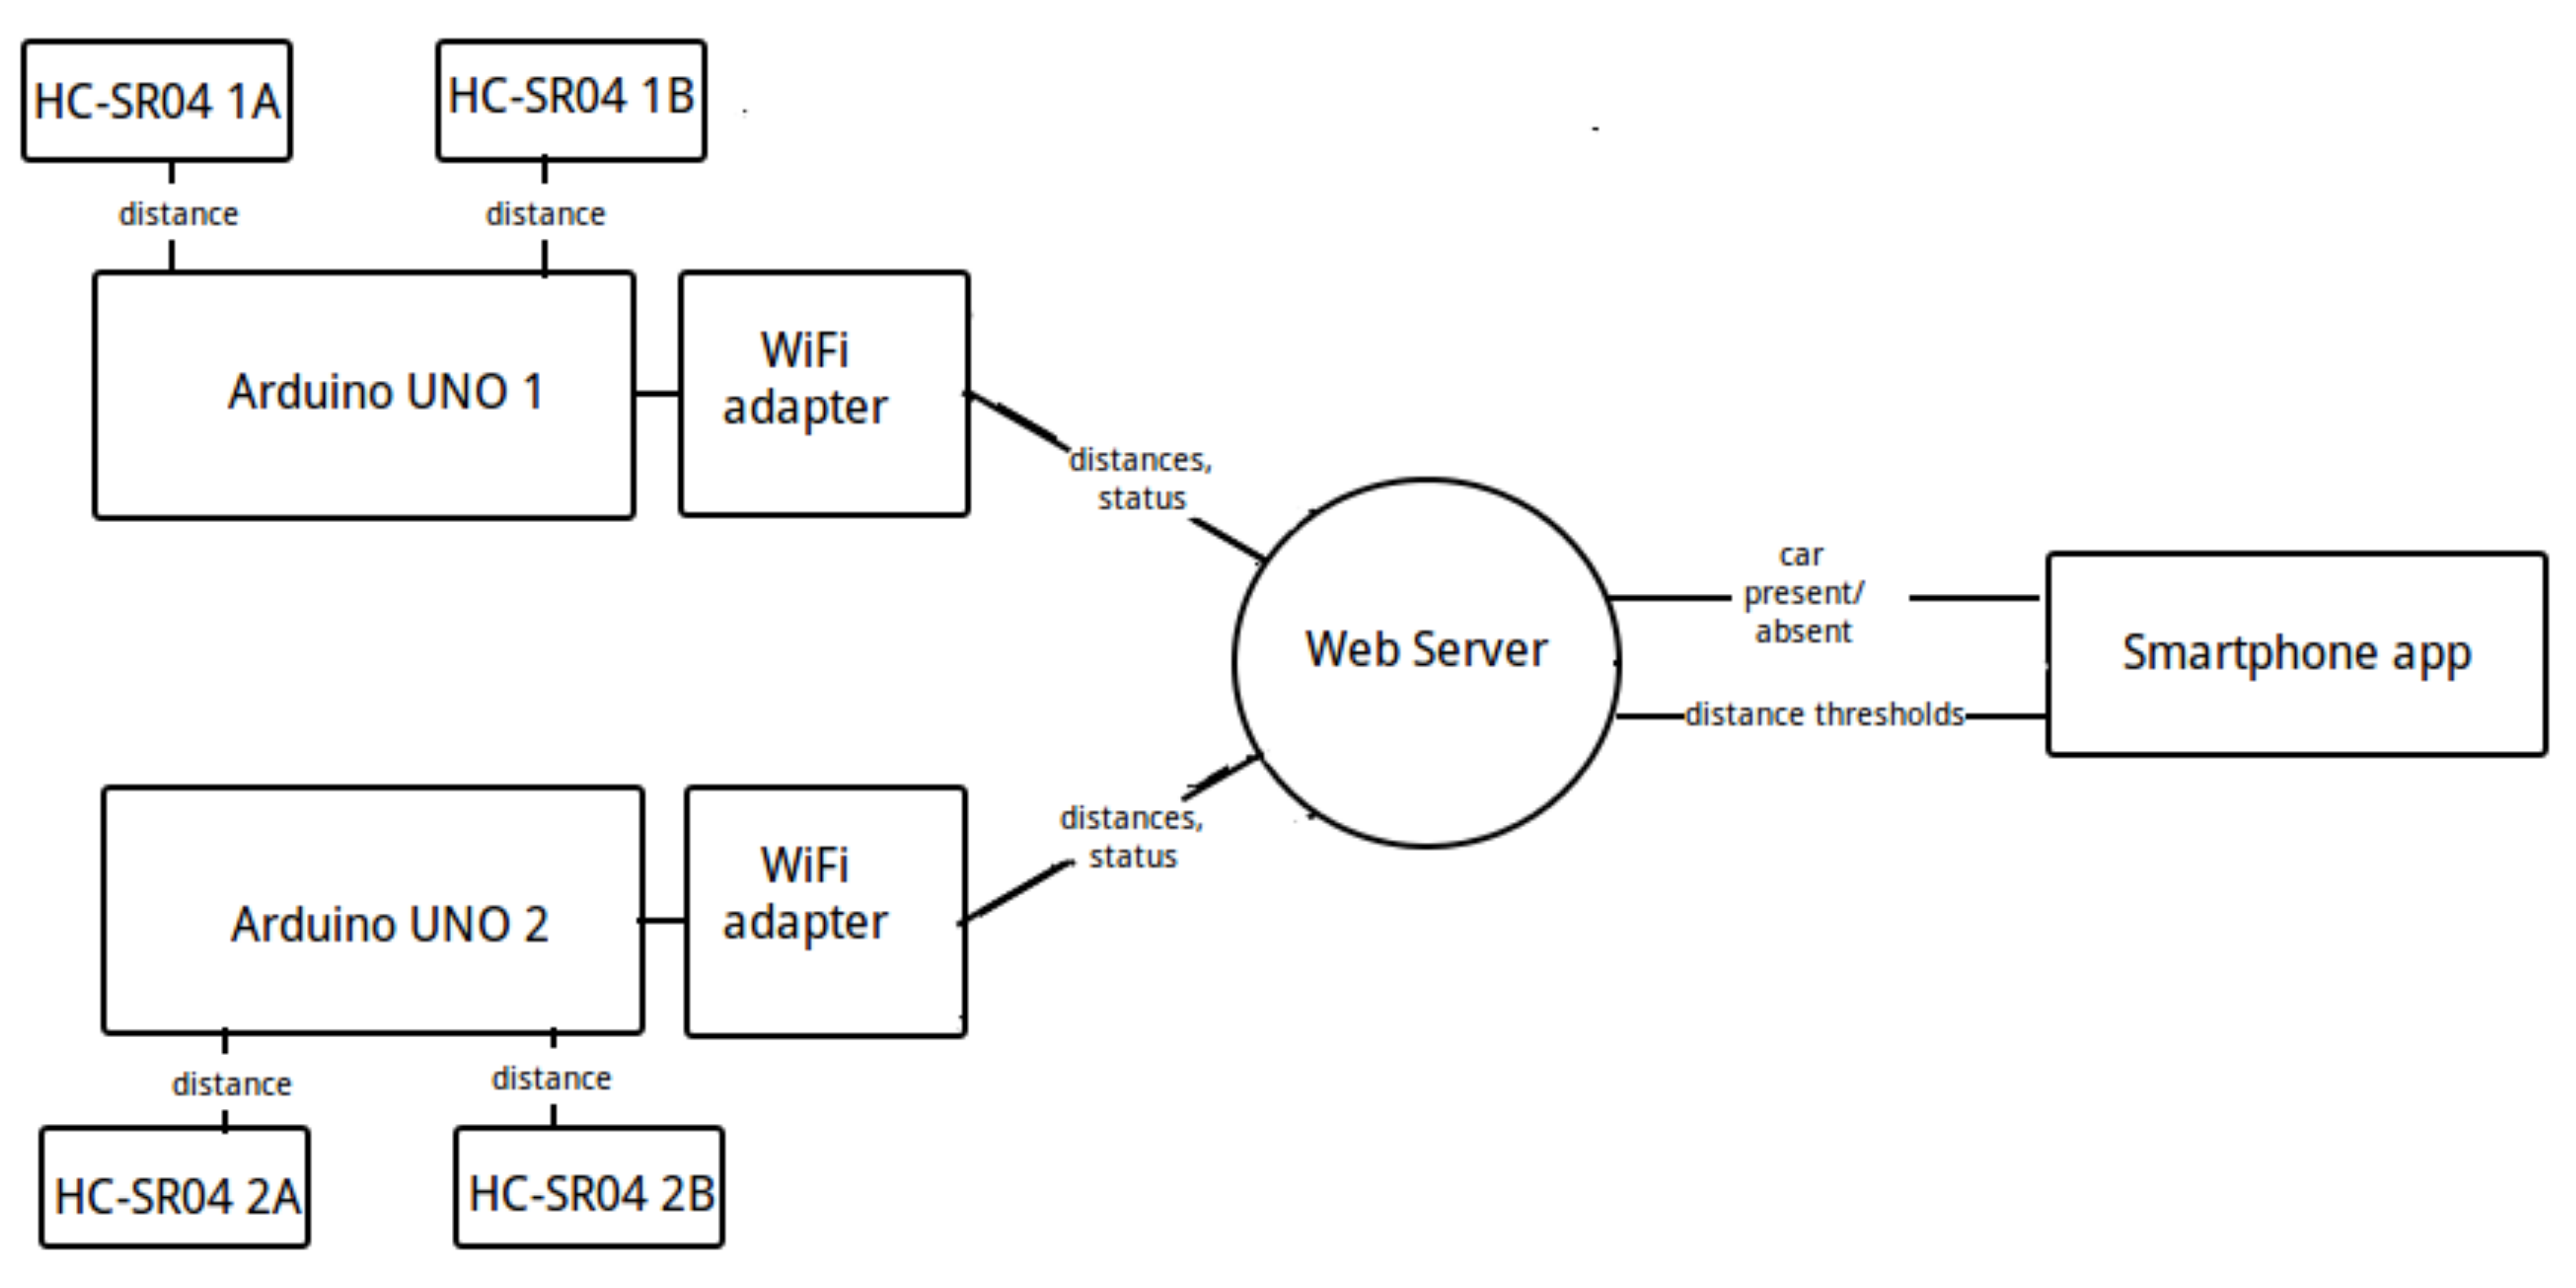
\includegraphics[width=3.0in]{block_diagram_0.png}
\caption{Block diagram of components used in our \texttt{CarSensor} prototype.}
\label{fig_blockdiagram}
\end{figure}

Each sensor module consists of two sensors, a microcontroller, and a network adapter. Each module is responsible for sensing two adjacent parking spaces, as shown in Figure~\ref{fig_curb}. The parking space in the middle of the figure is sensed by module 1's sensor B and module 2's sensor A; the parking space on the right would be sensed by module 2's sensor B and module 3's sensor A, and so on.
\begin{figure}[h]
\centering
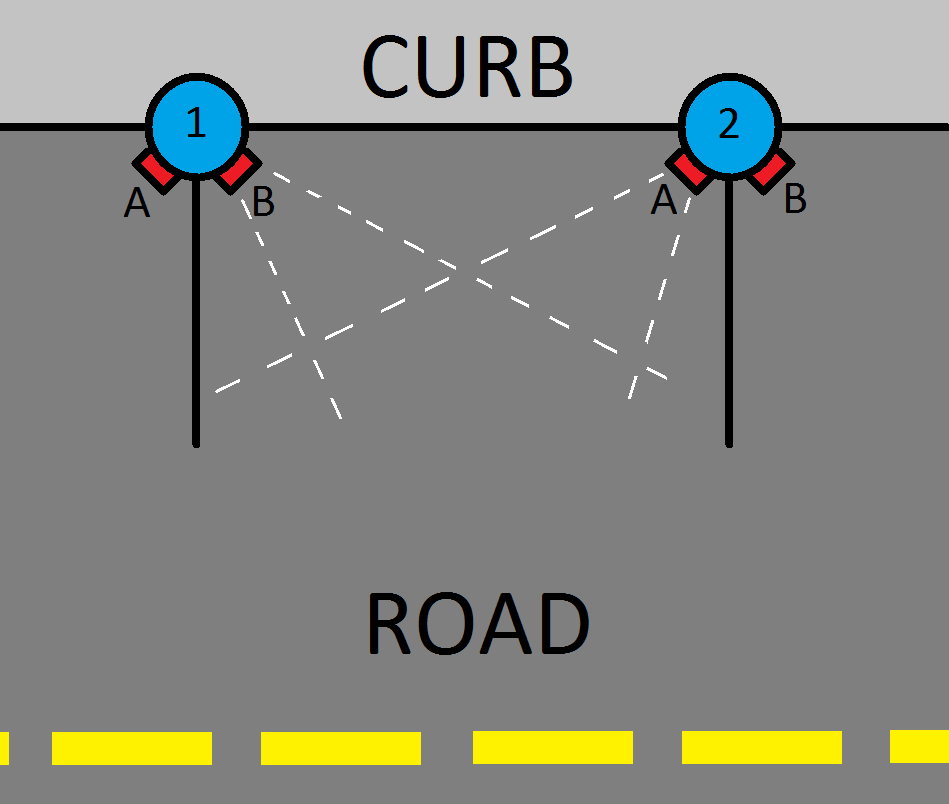
\includegraphics[width=2.0in]{parkingspace.png}
\caption{Physical layout of networked sensors used in \texttt{CarSensor}.}
\label{fig_curb}
\end{figure}

Each sensor module must also have a unique network identifier related to its physical location to allow the server to reason about the state of each parking space. In our prototype, we used IP addresses, but the limitations of that approach will be discussed in Section~\ref{sec_futurework}.

\section{Physical Layer}
Our prototype design was motivated by speed and ease of development: we selected components that were easy to get up and running, bearing in mind that we were only developing a prototype and not a production-ready system.

\subsection{Arduino UNO microcontroller}

\begin{figure}[h]
	\centering
	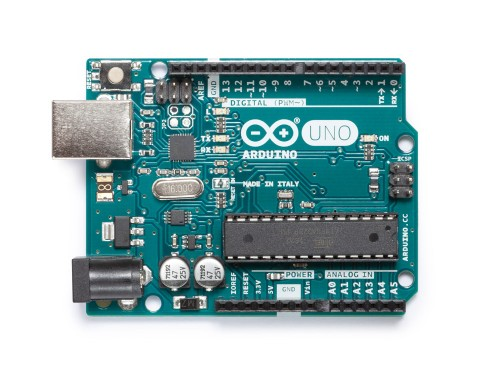
\includegraphics[width=2.5in]{arduinoUNO.jpg}
	\caption{Arduino UNO (image credit: Arduino)}
	\label{fig_arduinoUNO}
\end{figure}

Shown in Figure~\ref{fig_arduinoUNO}, the Arduino UNO is an open-source development board built around the ATmega328P microcontroller and has become a popular platform for prototyping simple embedded applications. We selected it for its overall ease of use due to its integrated development environment (IDE) and the large user base.

\subsection{HC-SR04 ultrasonic distance sensor}

\begin{figure}[h]
	\centering
	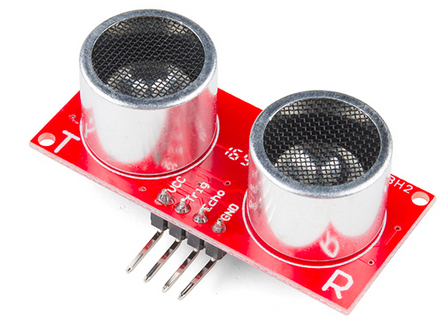
\includegraphics[width=2.0in]{hcsr04.png}
	\caption{HC-SR04 ultrasonic distance sensor (image credit: SparkFun Electronics \textsuperscript{\textregistered})}
	\label{fig_hcsr04}
\end{figure}

The HC-SR04 sensor, pictured in Figure~\ref{fig_hcsr04}, has two communication pins: \texttt{TRIG} (a digital input) and \texttt{ECHO} (a digital output). Its operational principle is similar to sonar: when \texttt{TRIG} is toggled high, the sensor emits an ultrasonic pulse; if an object reflects the pulse back to the sensor, it sets \texttt{ECHO} high. The microcontroller simply times the delay between setting \texttt{TRIG} high and receiving a logical 1 on \texttt{ECHO} and multiplies that time by the speed of sound (343 $\frac{\textrm{m}}{\textrm{s}}$ in air at sea level) to estimate how far away the object is.

\texttt{CarSensor} is more concerned with detecting the presence of a vehicle in a parking space than with measuring distance, so measurements made with the HC-SR04 are compared to a threshold. If the measured distance is less than the threshold, a \texttt{proximity} bit, specific to that sensor, is set to 1 and sent to the server via the WiFi adapter; otherwise, \texttt{proximity} is set to 0 and then sent to the server. Since each Arduino uses two HC-SR04 sensors, each Arduino sends two \texttt{proximity} bits to the server, delimited by a space. This transmission occurs at a regular frequency (0.5 Hz in our prototype); this will be expanded on in Section~\ref{sec_futurework}.

\subsection{ESP8266 WiFi adapter}

\begin{figure}[h]
	\centering
	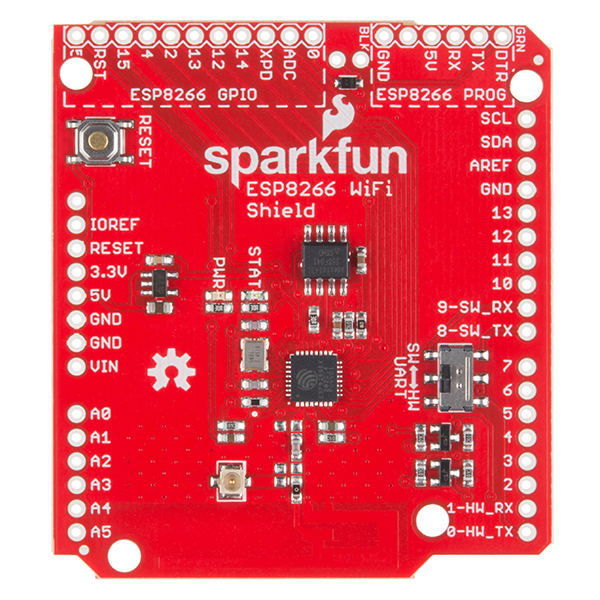
\includegraphics[width=2.0in]{esp8266.jpg}
	\caption{SparkFun ESP8266 WiFi shield for Arduino UNO (image credit: SparkFun Electronics \textsuperscript{\textregistered})}
	\label{fig_esp8266}
\end{figure}

After selecting our microcontroller, we needed to select a compatible WiFi adapter. We chose SparkFun's ESP8266 shield, pictured in Figure~\ref{fig_esp8266}, which is built around the ESP8266 system-on-a-chip (SoC) and provides TCP server and client functionality. It interfaces with the Arduino UNO over ``software serial'', leaving the Arduino UNO's hardware serial port available for other communication uses (debugging via a terminal emulator, in our case). We made use of SparkFun's Arduino library and starter code\footnote{\url{https://github.com/sparkfun/SparkFun_ESP8266_AT_Arduino_Library}} to accelerate the ESP8266's learning curve

\section{Network Layer}
\subsection{Sensor clients}
Using the ESP8266 in TCP client mode, each Arduino UNO sends proximity information from both HC-SR04 sensors to the server at 0.5 Hz.
\subsection{Server}
We used \texttt{Node.js}\textsuperscript{\textregistered}\footnote{\url{https://nodejs.org/en/}} to develop a rudimentary server to collect data from each sensor module and handle requests from the smartphone app. specifically, we used the \texttt{net}\footnote{\url{https://nodejs.org/api/net.html#net_net}} module to create an asynchronous streaming TCP server with that listens for requests on two ports (one for sensor modules, another for the smartphone app).
\subsubsection{TCP sockets}
Sensor modules communicate with the server on port 8080, and the smartphone app communicates with the server on port 8000. This decision was motivated by the need for a modular system; moreover, it simplifies the server design because TCP requests from the smartphone app do not need to be filtered out from sensor modules' TCP requests.
\subsubsection{State machine}
The core of \texttt{CarSensor} is a simple finite state machine (FSM) running on the server. As shown in Figure~\ref{fig_fsm}, the FSM has four states:
\begin{itemize}
\item \texttt{empty},
\item \texttt{pending full},
\item \texttt{full}, and
\item \texttt{pending empty}.
\end{itemize}
\begin{figure}[h]
	\centering
	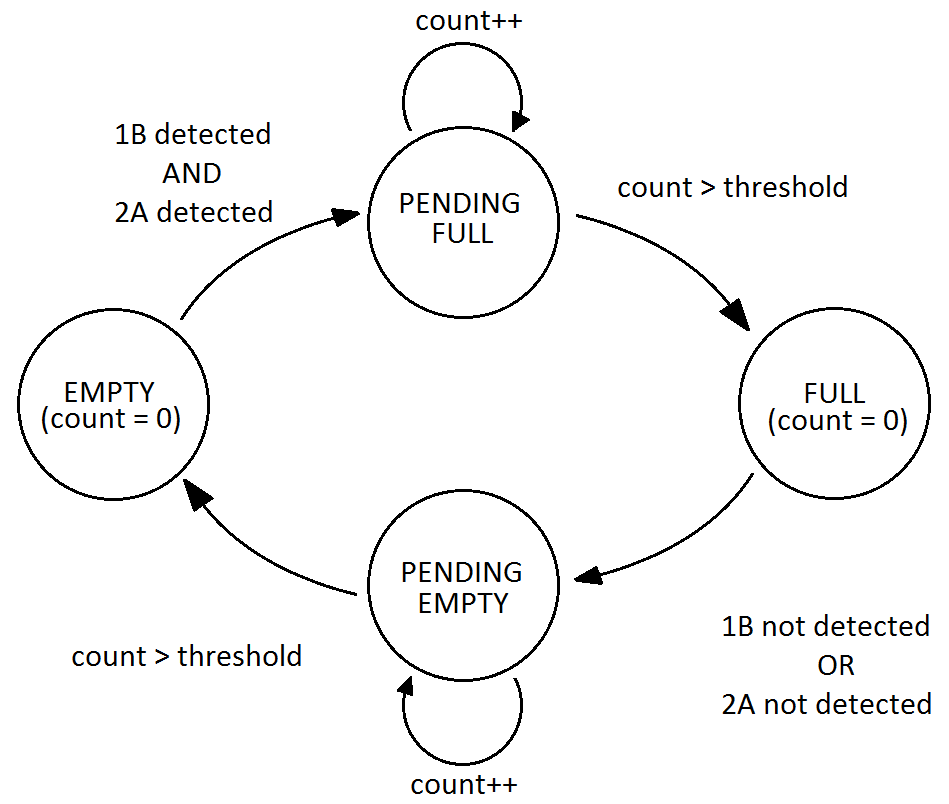
\includegraphics[width=2.5in]{FSM.png}
	\caption{Finite state machine for vehicle detection}
	\label{fig_fsm}
\end{figure}

A change in the \texttt{proximity} bits that correspond to a parking space triggers a transition from \texttt{empty} or \texttt{full} to one of the ``pending'' states. The FSM then uses a counter to determine when to transition from a ``pending'' state to \texttt{full} or \texttt{empty}. If the change persists until \texttt{count} reaches a \texttt{threshold} value, the state transitions; otherwise, it reverts to the state before the ``pending'' state.

\texttt{count} increments at the same rate that the sensor module sends new \texttt{proximity} data, so \texttt{threshold} represents a time duration. In our prototype, the value of \texttt{threshold} is 5, corresponding to 10 seconds.
\subsection{Smartphone app client}
\begin{figure}[h]
	\centering
	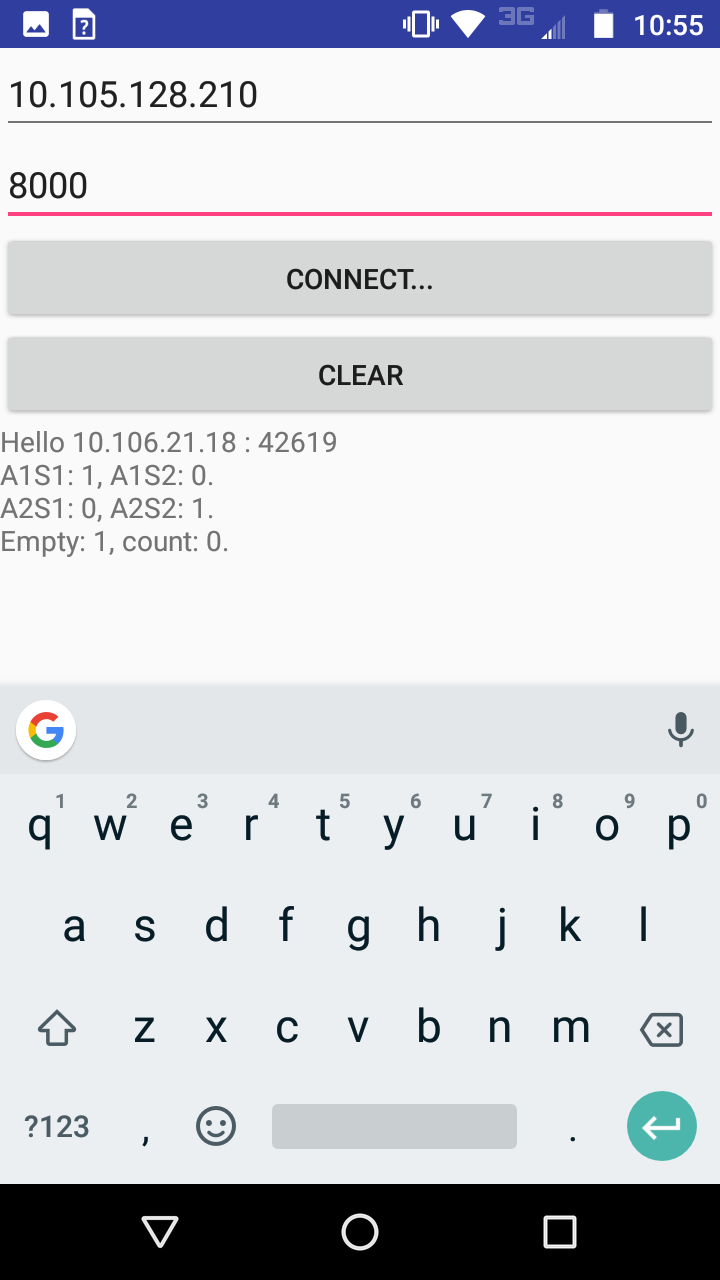
\includegraphics[width=2.0in]{app.png}
	\caption{Screenshot of the \texttt{CarSensor} Android app}
	\label{fig_app}
\end{figure}
\section{Future Work}\label{sec_futurework}
\subsection{Ease of use}
\subsection{Extensibility}
\subsection{Robustness}
\subsection{Power}
\subsection{Security}
\section{Conclusion}

\end{document}